%!TEX root = farm.tex

\section{Compiler and Debugging Environment}\label{sec:design}

This section describes the design and implementation of our compiler and
debugging environment for NVIDIA's GPU microcontrollers.

\subsection{Microcontroller}

\begin{table}[!t]
\caption{Specification of GF100 microcontroller.} 
\label{tab:fermi}
\hbox to\hsize{\hfil
\begin{tabular}{|l|r|r|}\hline
Name & HUB & GPC\\\hline
Number of units	& 1 & 4\\\hline
Bit & 32bit & 32bit\\\hline
Code size & 16,384 byte & 8,192 byte\\\hline
Data size & 4,096 byte & 2,048 byte\\\hline
\end{tabular}\hfil}
\end{table}

This paper presumes the microcontroller of NVIDIA's Fermi architecture.
In particular, we target the GeForce GTX 480 graphics card designed
based on the GF100 architecture.
In this architecture, a streaming multiprocessor (SM) consists of
32 CUDA cores, while a graphics processing cluster (GPC) consists of 4
SM's.
There are four GPC's in total equipped in the GF100 architecture, and
hence the maximum number of CUDA cores is 512.

Table~\ref{tab:fermi} illustrates the specification of the GF100
microcontroller.
There are two types of microcontrollers, HUB and GPC, relevant to CUDA
engines.
HUB is broadcasting the access to all GPC's, while the GPC represents a
specific microcontroller for each GPC engine.
Since the maximum code size is limited to 16KB as indicated in Table
\ref{tab:fermi}, developers should carefully design the firmware.

\subsection{Compiler Implementation}

\begin{figure*}[!t]
\begin{center}
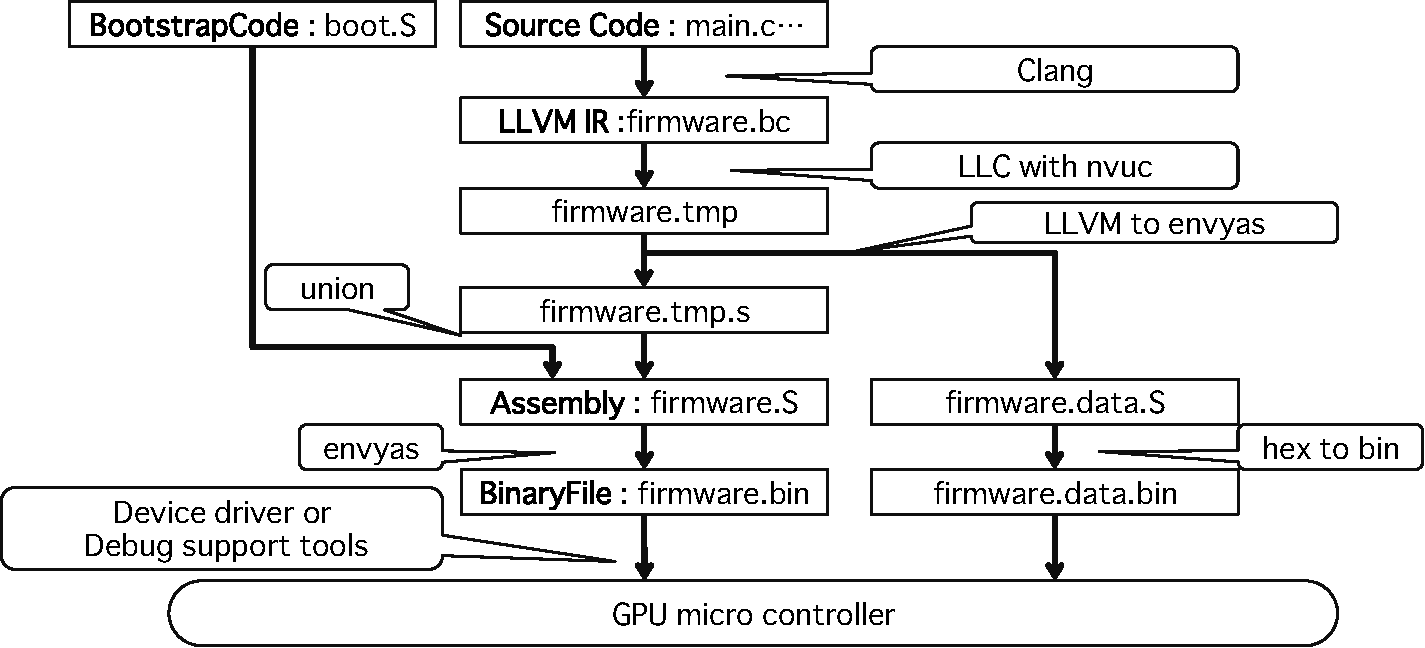
\includegraphics[width=12cm]{./img/step_compiler.pdf}
\end{center}
\caption{Overview of Compiler Implementation.}
\label{fig:compiler}
\end{figure*}

Figure \ref{fig:compiler} shows an overview of our compiler
implementation.
The main flow of compilation is done by Clang.
It generates the LLVM IR from the C source file.
The LLC next generates assembly code, which contains code and data in
separate files.
Finally, the Envytools outputs an executable file.
This executable file can be launched by the device driver, and can also
be tested by our debugging tool described in the later section.
To summarize, our compiler takes the following stages:

\begin{figure}[!t]
 \begin{center}
  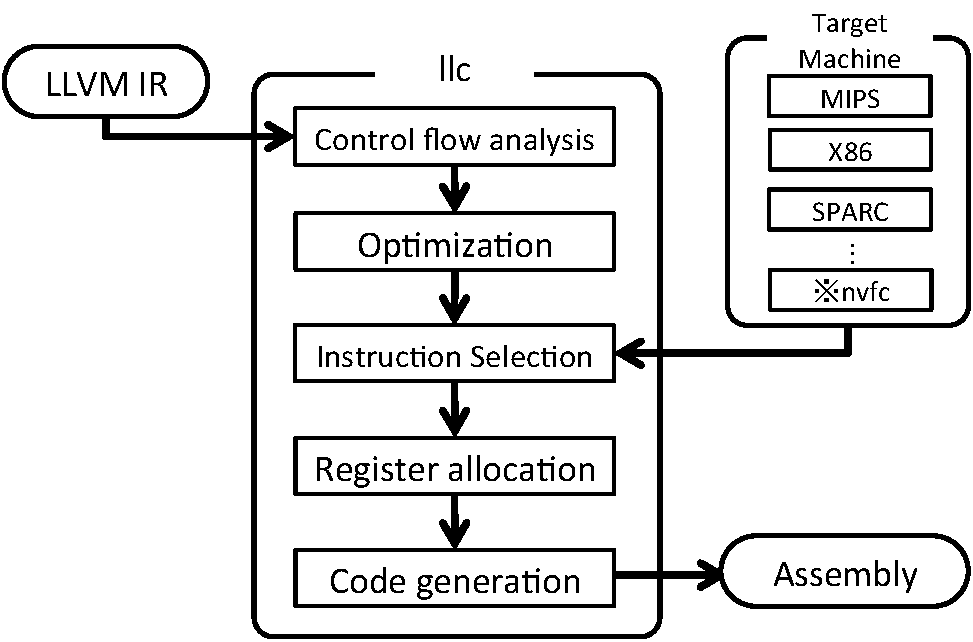
\includegraphics[width=6cm]{./img/llc.pdf}
 \end{center}
 \caption{Code generation stages of LLC.}
 \label{fig:llc}
\end{figure}

\begin{description}
\item[ (1) Clang]\mbox{}\\
	   This is a frontend of C language that generates LLVM IR code
	   from the source file.

\item[ (2) LLC with nvuc]\mbox{}\\
	   This is a backend of LLVM that compiles LLVM IR code into
	   assembly code. 
	   As shown in Figure~\ref{fig:llc}, there are five steps to
	   exploit compilation: (i) flow analysis, (ii) optimization,
	   (iii) instruction selection, (iv) register allocation, and
	   (v) code generation.
	   This flow is not dependent on the target machine.
	   The LLC reads a configuration of the target machine at the
	   time of instruction selection, and selects a set of the
	   instruction and register to meet the specifications of each
	   machine.
	   Our implementation adds a new configuration called nvuc
	   (NVIDIA Micro-Controller) to support NVIDIA's GPU
	   microcontrollers under LLVM.

\item[ (3) LLVM to envyas]\mbox{}\\
	   This stage divides the generated assembly code into code and
	   data sections so that we can create binary images using
	   ``envyas'', which is a microcontroller assembler provided by
	   the Envytools suite.
	   The bootstrap code is also unified into the binary images
	   in this stage.

\item[ (4) envyas]\mbox{}\\
	   This is a final assembly stage for the microcontroller, which
	   generates the byte code of the firmware.

\item[ (5) hex to bin]\mbox{}\\
	   This stage translates the hexadecimal byte code to the binary
	   format so that the firmware can execute on the
	   microcontroller.

\item[ (6) Running the microcontroller]\mbox{}\\
	   The compiled firmware is loaded on the microcontroller by the
	   device driver.
	   We also support a debugging tool that launches the firmware
	   in the same way as the device driver for development
	   purposes.
\end{description}

\subsection{Debugging Support}

\begin{figure}[!t]
 \begin{center}
  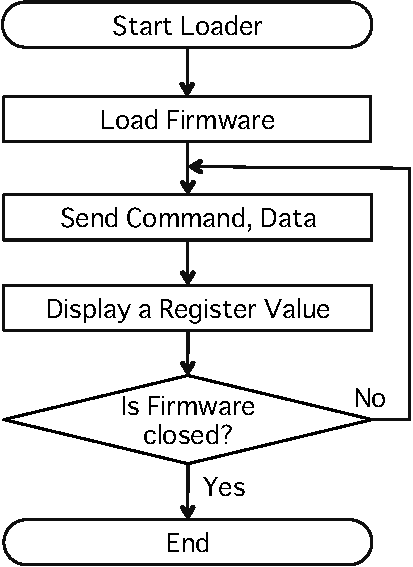
\includegraphics[width=3cm]{./img/loader.pdf}
 \end{center}
 \caption{Flowchart of our debugging tool.}
 \label{fig:loader}
\end{figure}

We support a debugging tool to load the firmware, send commands and
data, monitor the status, and display register and memory values of the
microcontroller.
Figure~\ref{fig:loader} shows control flow of our debugging tool.
The following are the details of each block in the flow:

\begin{description}
 \item[(1) Load Firmware]\mbox{}\\
	   Our debugging tool uploads a set of firmware programs on to
	   the HUB and the GPC microcontrollers.
	   The uploaded firmware programs start execution when a flag is
	   set in the specified register.
 \item[(2) Send Command and Data]\mbox{}\\
	    The microcontroller is event-driven.
	    It is totally suspended in an idle state.
	    When it receives a command from the debugging tool through
	    the PCI bus, the interrupt handler is invoked and its
	    execution is resumed.
\item[(3) Display Register Value] \mbox{}\\
	   The microcontroller has a set of registers that may be used
	   by the debugging tool for any purpose.
	   There are also several important registers relevant to
	   firmware execution.
	   The debugging tool hence displays the values of these
	   registers to notify what is happening.
\end{description}

\subsection{Firmware Development}

In this paper, we present the most basic firmware program for NVIDIA's
GPU microcontrollers.
We develop this firmware entirely using our compiler and debugging
environment.
This is indeed the initial step toward fine-grained GPU resource
management using microcontrollers, and enhanced functions could build
upon this work.

\begin{figure*}[!t]
 \begin{center}
  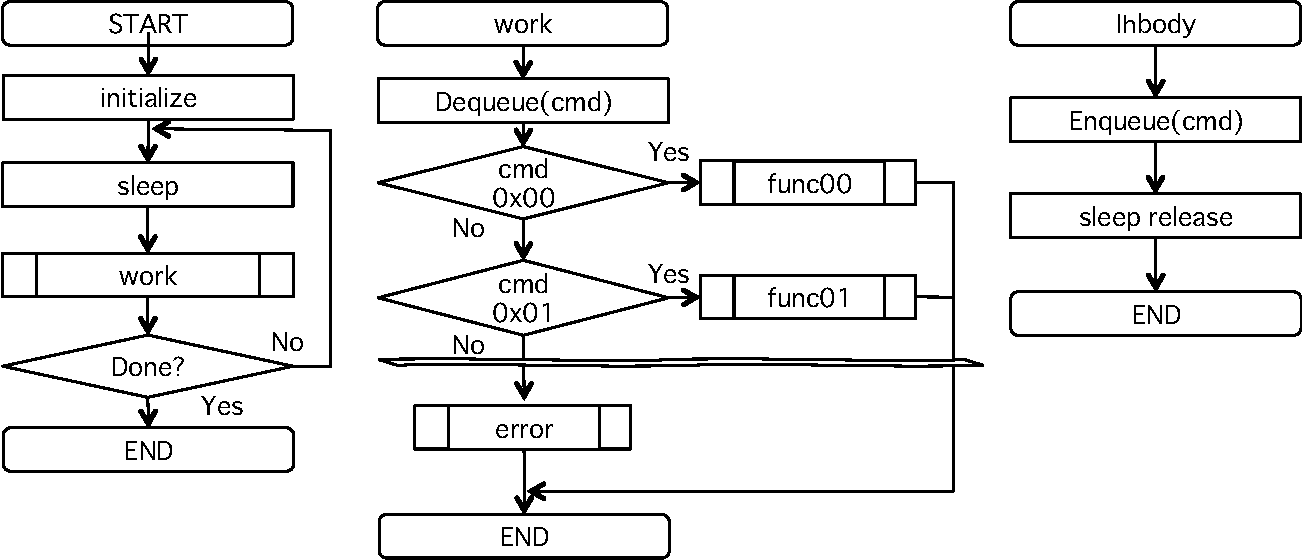
\includegraphics[width=12cm]{./img/firmware.pdf}
 \end{center}
 \caption{Flowchart of our basic firmware.}
 \label{fig:firmware}
\end{figure*}

Figure \ref{fig:firmware} shows control flow of the basic firmware
developed in this paper.
The following are the details of each block in the flow.

\begin{description}
 \item[(1) initialize]\mbox{}\\
	    The firmware configures the interrupt handler, and receives
	    the default set of data when started.
 \item[(2) sleep]\mbox{}\\
	    The firmware enters the standby mode in the main event loop,
	    waiting for the next command issued by the device driver or
	    the debugging tool.
	    Upon every arrival of the command, an interrupt is generated
	    on the microcontroller, awakening the firmware in the
	    ``ihbody'' function. 
 \item[(3) ihbody] \mbox{}\\
	    This is an interrupt handler invoked by the command.
	    All we have to do here is to enqueue the corresponding
	    command, and releases the standby mode to resume firmware
	    execution.
 \item[(4) work] \mbox{}\\
	    This is a main body of the firmware.
	    It is called when the firmware is released from the standby
	    mode.
	    The basic procedure of this function is to dequeue a pending
	    command one by one, and call the function corresponding to
	    the command.
	    If the specified flag is cleared, we destroy the firmware. 
\end{description}

